\section{Numerical experiments of facial recognition}
\subsection{Yale Face Database}
The experimentation reported on here was performed on the \textit{Extended Yale
Face Database B} \cite{yalefaceB}, consisting of 38 individuals (28 from the
extended database and 10 from the original one)\footnotemark. The first 36
people in the database is shown in Fig. \ref{Pall}.

\footnotetext{The database can be downloaded at \url{http://vision.ucsd.edu/~leekc/ExtYaleDatabase/ExtYaleB.html}}

\begin{figure}[h]
  \centering
  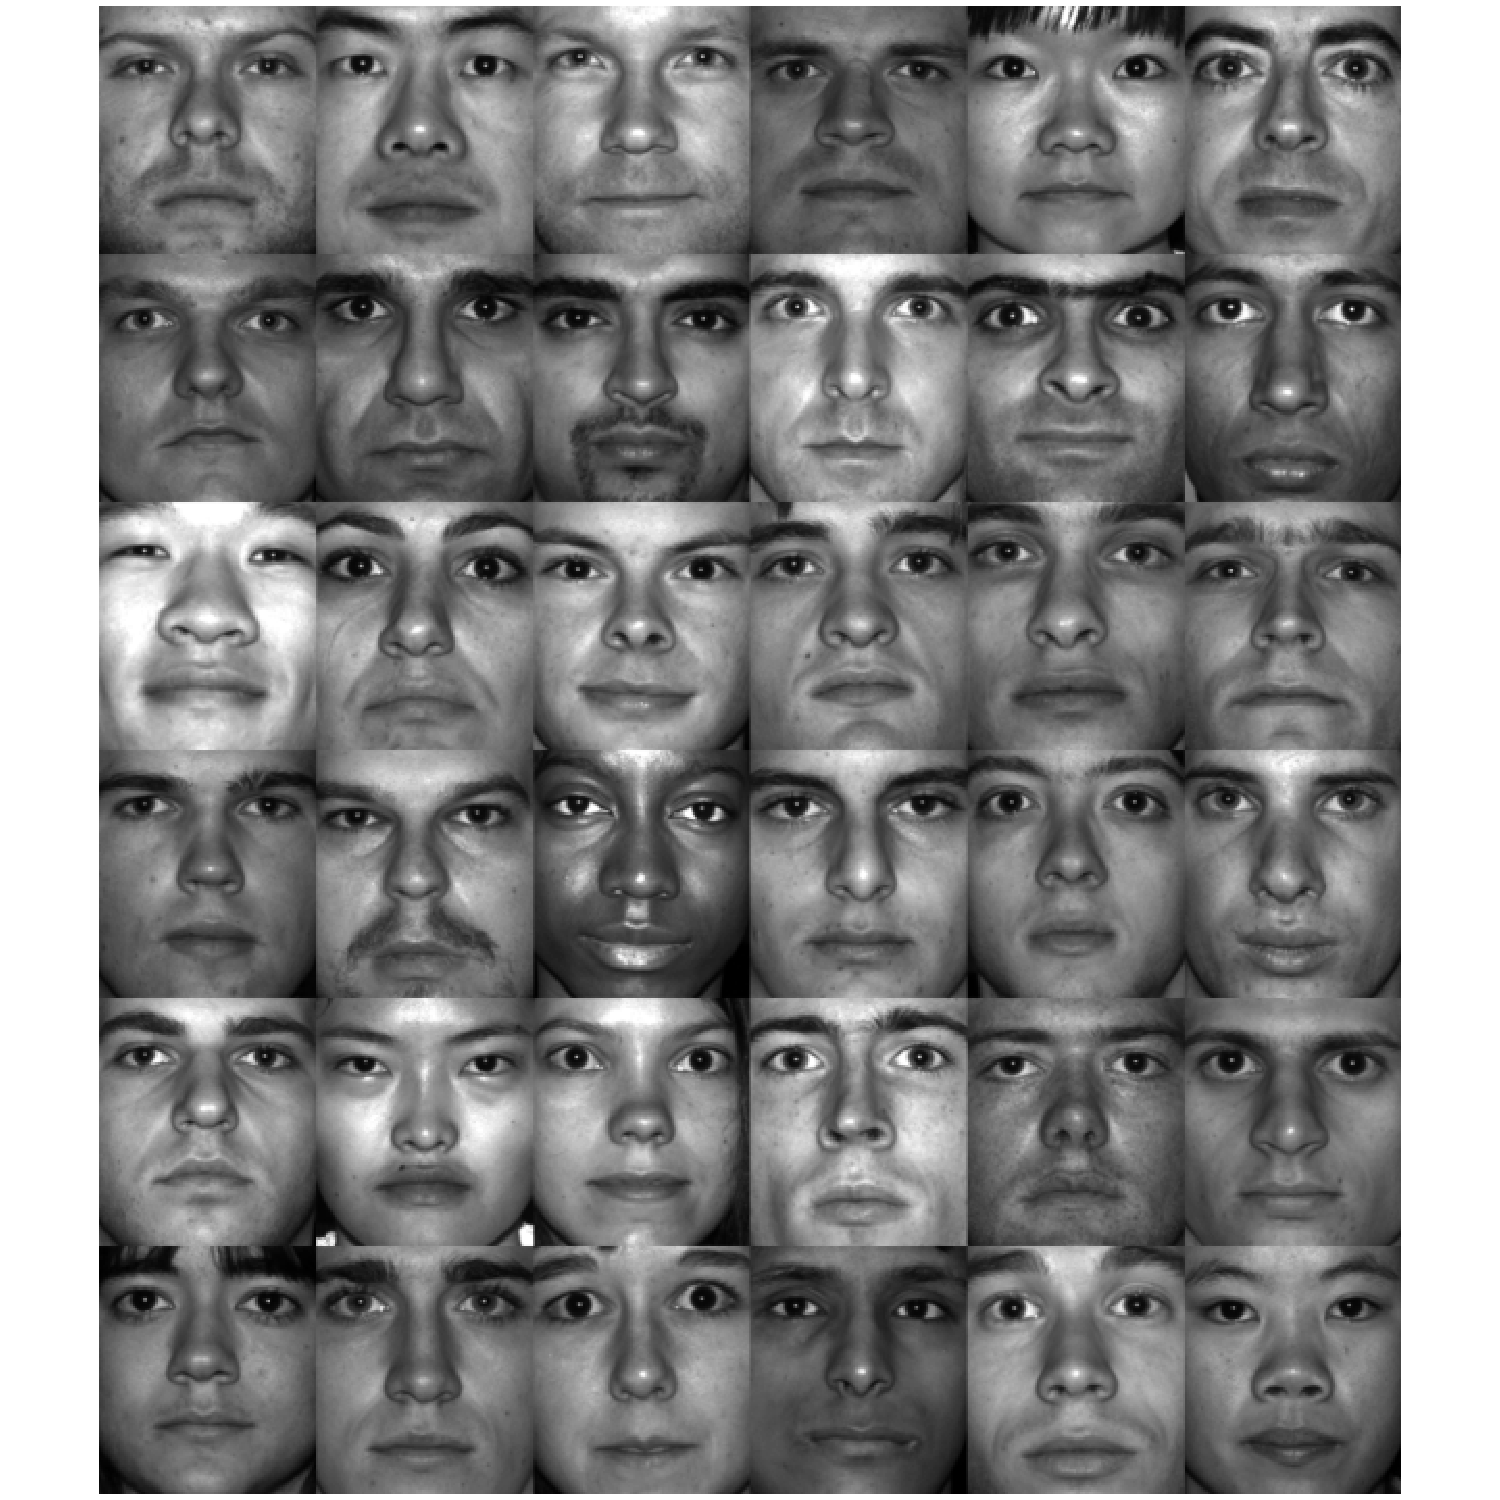
\includegraphics[width=\columnwidth]{Pall.pdf} 
  \caption{A single image for each person in the Yale database}
  \label{Pall}
\end{figure}

From each of the 38 individuals different portrait photos under 9 poses and 64
different lighting conditions were taken. The database was created with the help
of a geodesic dome with a lighting rig mounted at 64 different angles. While the
test person was sitting in the middle of the dome, within 2 seconds every light
was flashing, creating the variable illumination. An example of all 64 images of
one specific person can be found in appendix Fig. \ref{P01}.

As seen in \cite{yalefaceBcropped}, the photos were manually cropped to include
only the face with as little hair and background as possible. The images from
the frontal pose were aligned, (scaled and rotated) so that the eyes in each
image fell on the same positions lying on a horizontal line. Each image is 192
pixels tall and 168 pixels wide. For experimentation the images were vectorized,
meaning each 192$\times$168 image is represented by a vector containing 32,256
elements. 

I am using a subset of the dataset, only containing the first of 9 poses,
accounting for a total of 2410 images. As seen in Fig \ref{histogram}, Person 2,
5, 11--17 are missing some lighting conditions due to data corruption.
Nevertheless the dataset is quite balanced with almost every class represented
equally by 64 images. For the PCA feature extraction, I have used an already
preprocessed version dataset included in \cite{brunton2019data}. As Facebook's
DeepFace model expects input images as 3-channel RGB images, I had to first
resize and convert the grayscale portraits into RGB images using
OpenCV\cite{opencv_library}.

\begin{figure}[h]
  \centering
  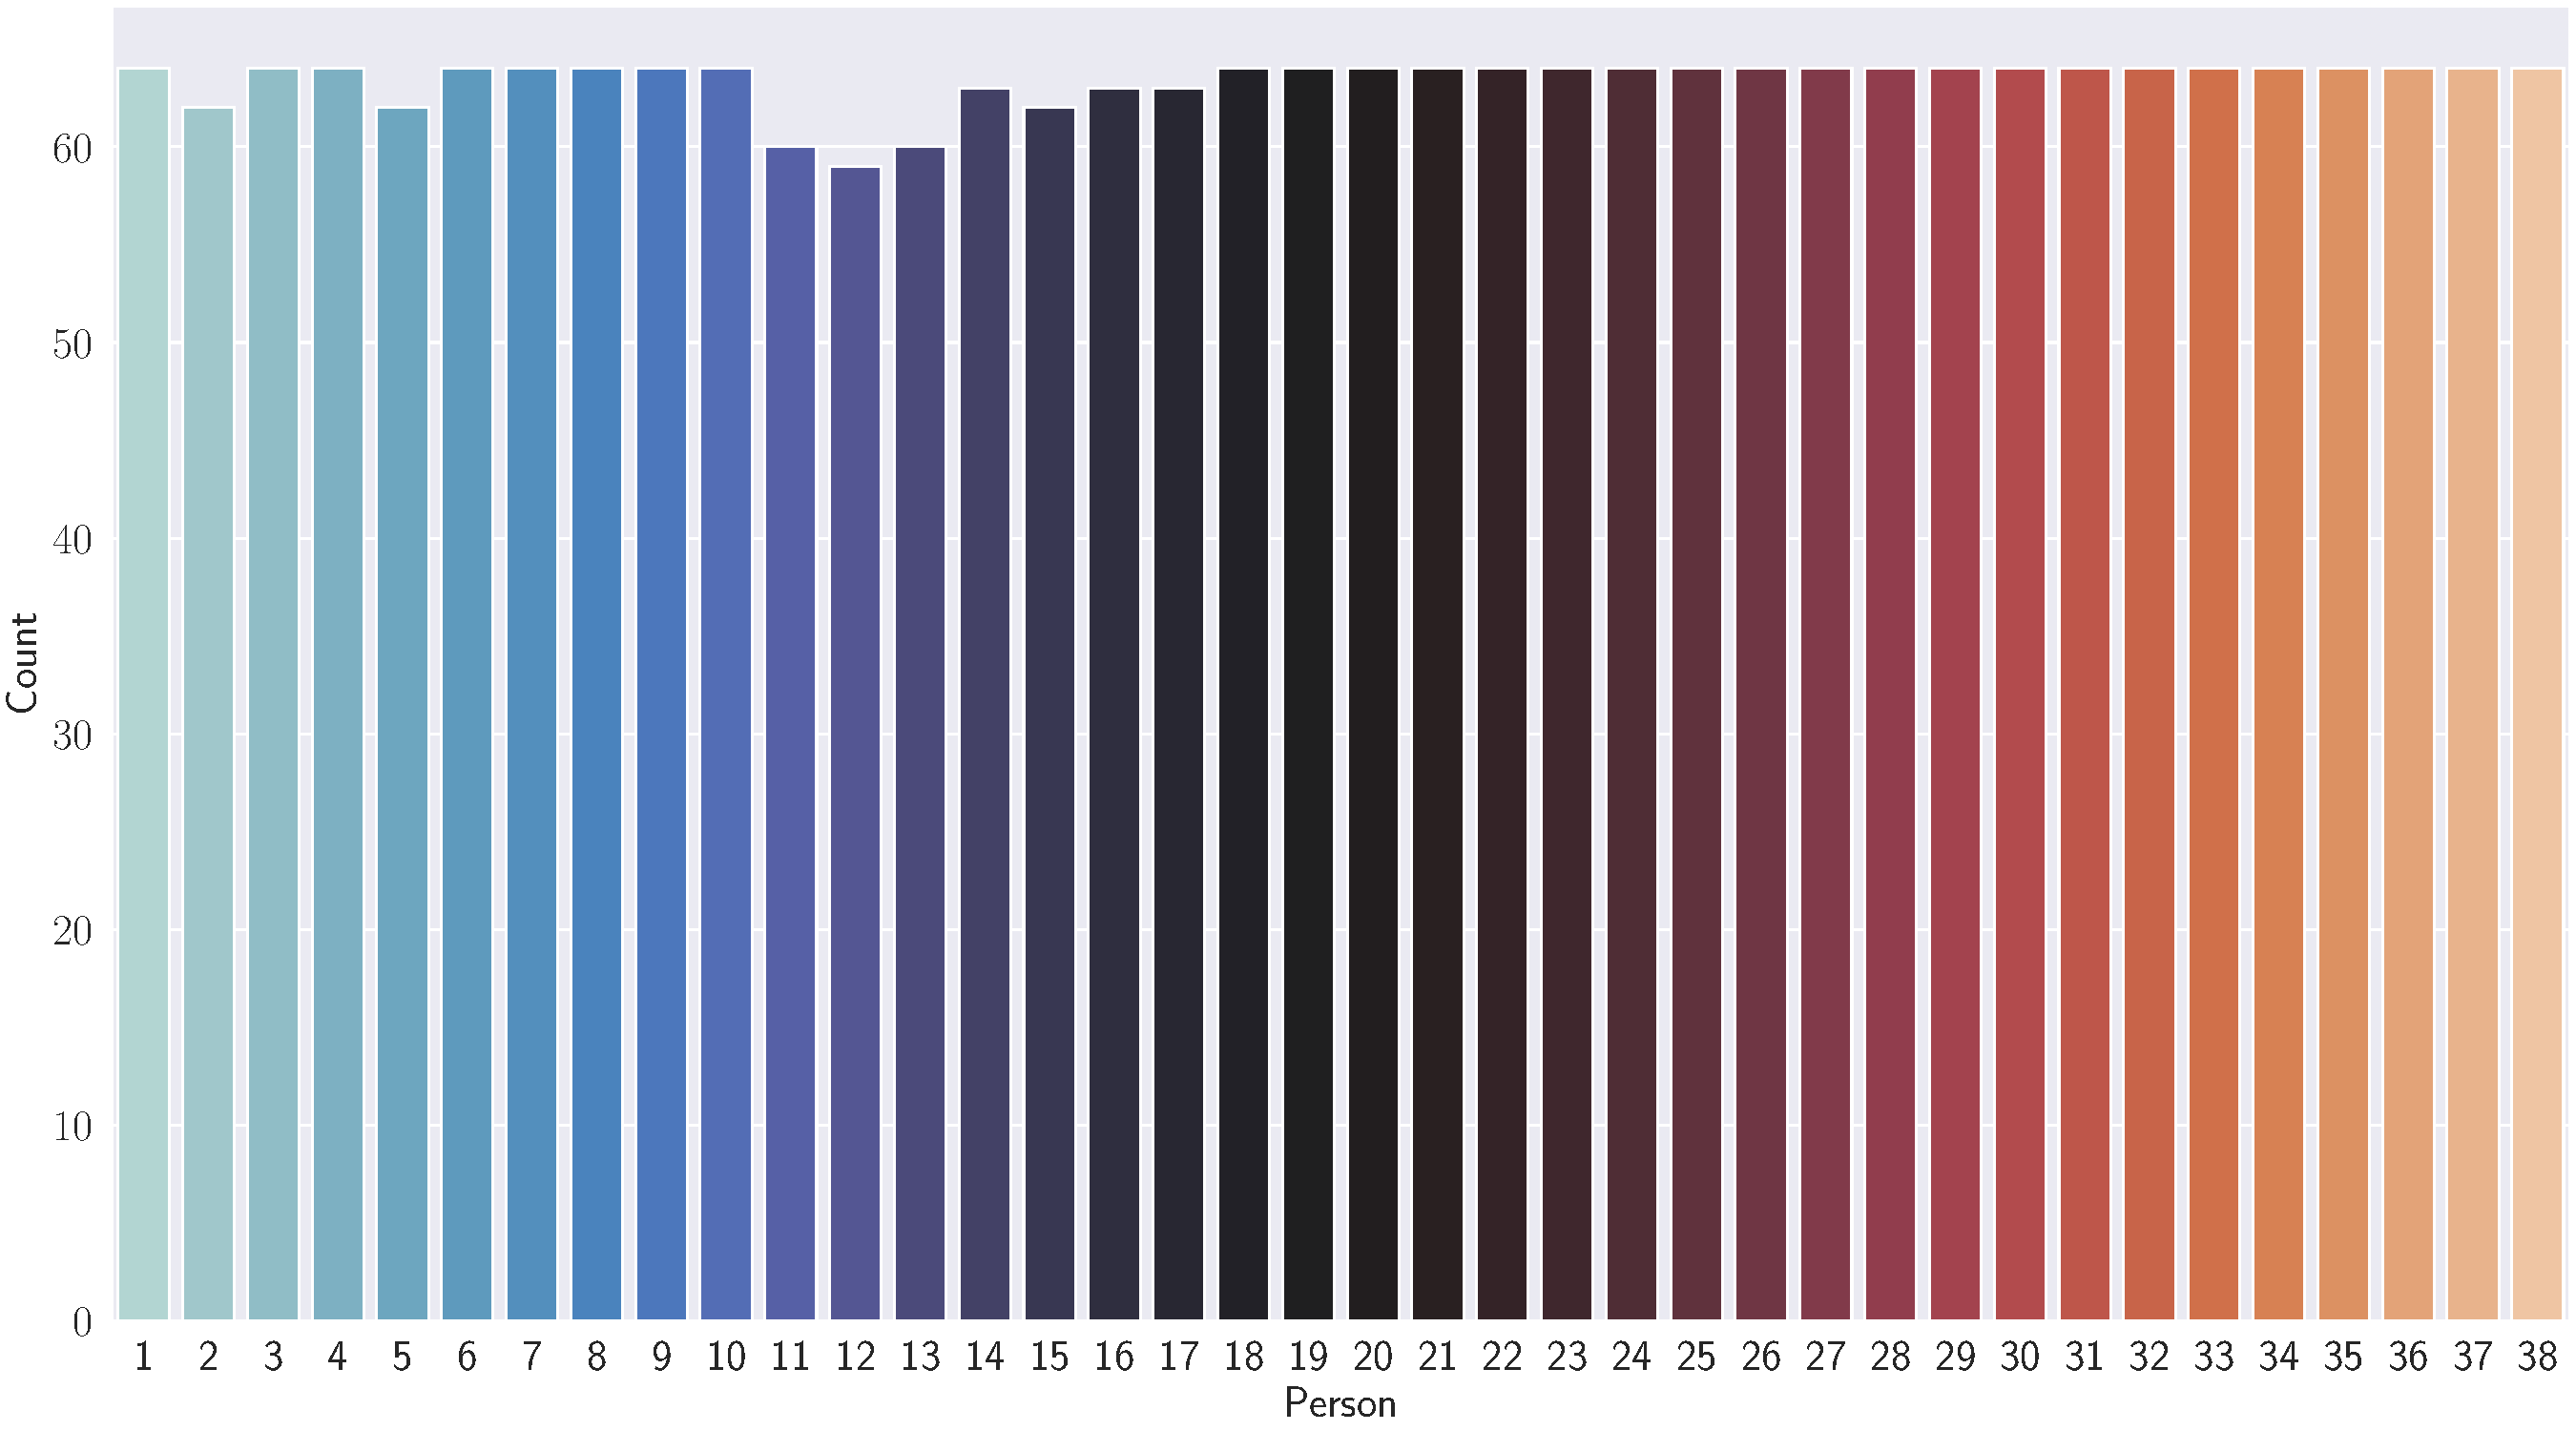
\includegraphics[width=\columnwidth]{histogram.pdf}
  \caption{Histogram showing how the dataset is distributed among the 38 classes}
  \label{histogram}
\end{figure}

